
%% bare_conf.tex
%% V1.4b
%% 2015/08/26
%% by Michael Shell
%% See:
%% http://www.michaelshell.org/
%% for current contact information.
%%
%% This is a skeleton file demonstrating the use of IEEEtran.cls
%% (requires IEEEtran.cls version 1.8b or later) with an IEEE
%% conference paper.
%%
%% Support sites:
%% http://www.michaelshell.org/tex/ieeetran/
%% http://www.ctan.org/pkg/ieeetran
%% and
%% http://www.ieee.org/

%%*************************************************************************
%% Legal Notice:
%% This code is offered as-is without any warranty either expressed or
%% implied; without even the implied warranty of MERCHANTABILITY or
%% FITNESS FOR A PARTICULAR PURPOSE! 
%% User assumes all risk.
%% In no event shall the IEEE or any contributor to this code be liable for
%% any damages or losses, including, but not limited to, incidental,
%% consequential, or any other damages, resulting from the use or misuse
%% of any information contained here.
%%
%% All comments are the opinions of their respective authors and are not
%% necessarily endorsed by the IEEE.
%%
%% This work is distributed under the LaTeX Project Public License (LPPL)
%% ( http://www.latex-project.org/ ) version 1.3, and may be freely used,
%% distributed and modified. A copy of the LPPL, version 1.3, is included
%% in the base LaTeX documentation of all distributions of LaTeX released
%% 2003/12/01 or later.
%% Retain all contribution notices and credits.
%% ** Modified files should be clearly indicated as such, including  **
%% ** renaming them and changing author support contact information. **
%%*************************************************************************


% *** Authors should verify (and, if needed, correct) their LaTeX system  ***
% *** with the testflow diagnostic prior to trusting their LaTeX platform ***
% *** with production work. The IEEE's font choices and paper sizes can   ***
% *** trigger bugs that do not appear when using other class files.       ***                          ***
% The testflow support page is at:
% http://www.michaelshell.org/tex/testflow/



\documentclass[conference]{IEEEtran}
% Some Computer Society conferences also require the compsoc mode option,
% but others use the standard conference format.
%
% If IEEEtran.cls has not been installed into the LaTeX system files,
% manually specify the path to it like:
% \documentclass[conference]{../sty/IEEEtran}





% Some very useful LaTeX packages include:
% (uncomment the ones you want to load)


% *** MISC UTILITY PACKAGES ***
%
%\usepackage{ifpdf}
% Heiko Oberdiek's ifpdf.sty is very useful if you need conditional
% compilation based on whether the output is pdf or dvi.
% usage:
% \ifpdf
%   % pdf code
% \else
%   % dvi code
% \fi
% The latest version of ifpdf.sty can be obtained from:
% http://www.ctan.org/pkg/ifpdf
% Also, note that IEEEtran.cls V1.7 and later provides a builtin
% \ifCLASSINFOpdf conditional that works the same way.
% When switching from latex to pdflatex and vice-versa, the compiler may
% have to be run twice to clear warning/error messages.






% *** CITATION PACKAGES ***
%
\usepackage{cite}
% cite.sty was written by Donald Arseneau
% V1.6 and later of IEEEtran pre-defines the format of the cite.sty package
% \cite{} output to follow that of the IEEE. Loading the cite package will
% result in citation numbers being automatically sorted and properly
% "compressed/ranged". e.g., [1], [9], [2], [7], [5], [6] without using
% cite.sty will become [1], [2], [5]--[7], [9] using cite.sty. cite.sty's
% \cite will automatically add leading space, if needed. Use cite.sty's
% noadjust option (cite.sty V3.8 and later) if you want to turn this off
% such as if a citation ever needs to be enclosed in parenthesis.
% cite.sty is already installed on most LaTeX systems. Be sure and use
% version 5.0 (2009-03-20) and later if using hyperref.sty.
% The latest version can be obtained at:
% http://www.ctan.org/pkg/cite
% The documentation is contained in the cite.sty file itself.






% *** GRAPHICS RELATED PACKAGES ***
%
\ifCLASSINFOpdf
   \usepackage[pdftex]{graphicx}
  % declare the path(s) where your graphic files are
   \graphicspath{{./images/}}
  % and their extensions so you won't have to specify these with
  % every instance of \includegraphics
   \DeclareGraphicsExtensions{.pdf}
\else
  % or other class option (dvipsone, dvipdf, if not using dvips). graphicx
  % will default to the driver specified in the system graphics.cfg if no
  % driver is specified.
  % \usepackage[dvips]{graphicx}
  % declare the path(s) where your graphic files are
  % \graphicspath{{../eps/}}
  % and their extensions so you won't have to specify these with
  % every instance of \includegraphics
  % \DeclareGraphicsExtensions{.eps}
\fi
% graphicx was written by David Carlisle and Sebastian Rahtz. It is
% required if you want graphics, photos, etc. graphicx.sty is already
% installed on most LaTeX systems. The latest version and documentation
% can be obtained at: 
% http://www.ctan.org/pkg/graphicx
% Another good source of documentation is "Using Imported Graphics in
% LaTeX2e" by Keith Reckdahl which can be found at:
% http://www.ctan.org/pkg/epslatex
%
% latex, and pdflatex in dvi mode, support graphics in encapsulated
% postscript (.eps) format. pdflatex in pdf mode supports graphics
% in .pdf, .jpeg, .png and .mps (metapost) formats. Users should ensure
% that all non-photo figures use a vector format (.eps, .pdf, .mps) and
% not a bitmapped formats (.jpeg, .png). The IEEE frowns on bitmapped formats
% which can result in "jaggedy"/blurry rendering of lines and letters as
% well as large increases in file sizes.
%
% You can find documentation about the pdfTeX application at:
% http://www.tug.org/applications/pdftex





% *** MATH PACKAGES ***
%
\usepackage{amsmath}
% A popular package from the American Mathematical Society that provides
% many useful and powerful commands for dealing with mathematics.
%
% Note that the amsmath package sets \interdisplaylinepenalty to 10000
% thus preventing page breaks from occurring within multiline equations. Use:
%\interdisplaylinepenalty=2500
% after loading amsmath to restore such page breaks as IEEEtran.cls normally
% does. amsmath.sty is already installed on most LaTeX systems. The latest
% version and documentation can be obtained at:
% http://www.ctan.org/pkg/amsmath

\usepackage{amssymb}



% *** SPECIALIZED LIST PACKAGES ***
%
\usepackage{algorithmic}
\usepackage{algorithm}
% algorithmic.sty was written by Peter Williams and Rogerio Brito.
% This package provides an algorithmic environment fo describing algorithms.
% You can use the algorithmic environment in-text or within a figure
% environment to provide for a floating algorithm. Do NOT use the algorithm
% floating environment provided by algorithm.sty (by the same authors) or
% algorithm2e.sty (by Christophe Fiorio) as the IEEE does not use dedicated
% algorithm float types and packages that provide these will not provide
% correct IEEE style captions. The latest version and documentation of
% algorithmic.sty can be obtained at:
% http://www.ctan.org/pkg/algorithms
% Also of interest may be the (relatively newer and more customizable)
% algorithmicx.sty package by Szasz Janos:
% http://www.ctan.org/pkg/algorithmicx




% *** ALIGNMENT PACKAGES ***
%
%\usepackage{array}
% Frank Mittelbach's and David Carlisle's array.sty patches and improves
% the standard LaTeX2e array and tabular environments to provide better
% appearance and additional user controls. As the default LaTeX2e table
% generation code is lacking to the point of almost being broken with
% respect to the quality of the end results, all users are strongly
% advised to use an enhanced (at the very least that provided by array.sty)
% set of table tools. array.sty is already installed on most systems. The
% latest version and documentation can be obtained at:
% http://www.ctan.org/pkg/array


% IEEEtran contains the IEEEeqnarray family of commands that can be used to
% generate multiline equations as well as matrices, tables, etc., of high
% quality.




% *** SUBFIGURE PACKAGES ***
%\ifCLASSOPTIONcompsoc
%  \usepackage[caption=false,font=normalsize,labelfont=sf,textfont=sf]{subfig}
%\else
%  \usepackage[caption=false,font=footnotesize]{subfig}
%\fi
% subfig.sty, written by Steven Douglas Cochran, is the modern replacement
% for subfigure.sty, the latter of which is no longer maintained and is
% incompatible with some LaTeX packages including fixltx2e. However,
% subfig.sty requires and automatically loads Axel Sommerfeldt's caption.sty
% which will override IEEEtran.cls' handling of captions and this will result
% in non-IEEE style figure/table captions. To prevent this problem, be sure
% and invoke subfig.sty's "caption=false" package option (available since
% subfig.sty version 1.3, 2005/06/28) as this is will preserve IEEEtran.cls
% handling of captions.
% Note that the Computer Society format requires a larger sans serif font
% than the serif footnote size font used in traditional IEEE formatting
% and thus the need to invoke different subfig.sty package options depending
% on whether compsoc mode has been enabled.
%
% The latest version and documentation of subfig.sty can be obtained at:
% http://www.ctan.org/pkg/subfig




% *** FLOAT PACKAGES ***
%
%\usepackage{fixltx2e}
% fixltx2e, the successor to the earlier fix2col.sty, was written by
% Frank Mittelbach and David Carlisle. This package corrects a few problems
% in the LaTeX2e kernel, the most notable of which is that in current
% LaTeX2e releases, the ordering of single and double column floats is not
% guaranteed to be preserved. Thus, an unpatched LaTeX2e can allow a
% single column figure to be placed prior to an earlier double column
% figure.
% Be aware that LaTeX2e kernels dated 2015 and later have fixltx2e.sty's
% corrections already built into the system in which case a warning will
% be issued if an attempt is made to load fixltx2e.sty as it is no longer
% needed.
% The latest version and documentation can be found at:
% http://www.ctan.org/pkg/fixltx2e


%\usepackage{stfloats}
% stfloats.sty was written by Sigitas Tolusis. This package gives LaTeX2e
% the ability to do double column floats at the bottom of the page as well
% as the top. (e.g., "\begin{figure*}[!b]" is not normally possible in
% LaTeX2e). It also provides a command:
%\fnbelowfloat
% to enable the placement of footnotes below bottom floats (the standard
% LaTeX2e kernel puts them above bottom floats). This is an invasive package
% which rewrites many portions of the LaTeX2e float routines. It may not work
% with other packages that modify the LaTeX2e float routines. The latest
% version and documentation can be obtained at:
% http://www.ctan.org/pkg/stfloats
% Do not use the stfloats baselinefloat ability as the IEEE does not allow
% \baselineskip to stretch. Authors submitting work to the IEEE should note
% that the IEEE rarely uses double column equations and that authors should try
% to avoid such use. Do not be tempted to use the cuted.sty or midfloat.sty
% packages (also by Sigitas Tolusis) as the IEEE does not format its papers in
% such ways.
% Do not attempt to use stfloats with fixltx2e as they are incompatible.
% Instead, use Morten Hogholm'a dblfloatfix which combines the features
% of both fixltx2e and stfloats:
%
% \usepackage{dblfloatfix}
% The latest version can be found at:
% http://www.ctan.org/pkg/dblfloatfix




% *** PDF, URL AND HYPERLINK PACKAGES ***
%
%\usepackage{url}
% url.sty was written by Donald Arseneau. It provides better support for
% handling and breaking URLs. url.sty is already installed on most LaTeX
% systems. The latest version and documentation can be obtained at:
% http://www.ctan.org/pkg/url
% Basically, \url{my_url_here}.




% *** Do not adjust lengths that control margins, column widths, etc. ***
% *** Do not use packages that alter fonts (such as pslatex).         ***
% There should be no need to do such things with IEEEtran.cls V1.6 and later.
% (Unless specifically asked to do so by the journal or conference you plan
% to submit to, of course. )


% correct bad hyphenation here
\hyphenation{op-tical net-works semi-conduc-tor}

%------------------------Thilo Package Area-----------------------------
%Package for writing german letters
\usepackage[utf8]{inputenc}

%-----------------------------------------------------------------------
\begin{document}
%
% paper title
% Titles are generally capitalized except for words such as a, an, and, as,
% at, but, by, for, in, nor, of, on, or, the, to and up, which are usually
% not capitalized unless they are the first or last word of the title.
% Linebreaks \\ can be used within to get better formatting as desired.
% Do not put math or special symbols in the title.
\title{Describing the role of Artificial Neural Networks in Reinforcement Learning}


% author names and affiliations
% use a multiple column layout for up to three different
% affiliations
\author{\IEEEauthorblockN{Thilo Stegemann}
\IEEEauthorblockA{University of Applied Sciences\\Applied Computer Science\\
12459 Berlin, Wilhelminenhofstraße 75A\\
Email: t.stegemann@gmx.de}}

% conference papers do not typically use \thanks and this command
% is locked out in conference mode. If really needed, such as for
% the acknowledgment of grants, issue a \IEEEoverridecommandlockouts
% after \documentclass

% for over three affiliations, or if they all won't fit within the width
% of the page, use this alternative format:
% 
%\author{\IEEEauthorblockN{Michael Shell\IEEEauthorrefmark{1},
%Homer Simpson\IEEEauthorrefmark{2},
%James Kirk\IEEEauthorrefmark{3}, 
%Montgomery Scott\IEEEauthorrefmark{3} and
%Eldon Tyrell\IEEEauthorrefmark{4}}
%\IEEEauthorblockA{\IEEEauthorrefmark{1}School of Electrical and Computer Engineering\\
%Georgia Institute of Technology,
%Atlanta, Georgia 30332--0250\\ Email: see http://www.michaelshell.org/contact.html}
%\IEEEauthorblockA{\IEEEauthorrefmark{2}Twentieth Century Fox, Springfield, USA\\
%Email: homer@thesimpsons.com}
%\IEEEauthorblockA{\IEEEauthorrefmark{3}Starfleet Academy, San Francisco, California 96678-2391\\
%Telephone: (800) 555--1212, Fax: (888) 555--1212}
%\IEEEauthorblockA{\IEEEauthorrefmark{4}Tyrell Inc., 123 Replicant Street, Los Angeles, California 90210--4321}}




% use for special paper notices
%\IEEEspecialpapernotice{(Invited Paper)}




% make the title area
\maketitle

% enables page numbering
\thispagestyle{plain}
\pagestyle{plain}

% As a general rule, do not put math, special symbols or citations
% in the abstract
\begin{abstract}
 TODO : Write an awesome abstract at the end!
\end{abstract}

% no keywords




% For peer review papers, you can put extra information on the cover
% page as needed:
% \ifCLASSOPTIONpeerreview
% \begin{center} \bfseries EDICS Category: 3-BBND \end{center}
% \fi
%
% For peerreview papers, this IEEEtran command inserts a page break and
% creates the second title. It will be ignored for other modes.
\IEEEpeerreviewmaketitle

% An example of a floating figure using the graphicx package.
% Note that \label must occur AFTER (or within) \caption.
% For figures, \caption should occur after the \includegraphics.
% Note that IEEEtran v1.7 and later has special internal code that
% is designed to preserve the operation of \label within \caption
% even when the captionsoff option is in effect. However, because
% of issues like this, it may be the safest practice to put all your
% \label just after \caption rather than within \caption{}.
%
% Reminder: the "draftcls" or "draftclsnofoot", not "draft", class
% option should be used if it is desired that the figures are to be
% displayed while in draft mode.
%
%\begin{figure}[!t]
%\centering
%\includegraphics[width=2.5in]{myfigure}
% where an .eps filename suffix will be assumed under latex, 
% and a .pdf suffix will be assumed for pdflatex; or what has been declared
% via \DeclareGraphicsExtensions.
%\caption{Simulation results for the network.}
%\label{fig_sim}
%\end{figure}

% Note that the IEEE typically puts floats only at the top, even when this
% results in a large percentage of a column being occupied by floats.


% An example of a double column floating figure using two subfigures.
% (The subfig.sty package must be loaded for this to work.)
% The subfigure \label commands are set within each subfloat command,
% and the \label for the overall figure must come after \caption.
% \hfil is used as a separator to get equal spacing.
% Watch out that the combined width of all the subfigures on a 
% line do not exceed the text width or a line break will occur.
%
%\begin{figure*}[!t]
%\centering
%\subfloat[Case I]{\includegraphics[width=2.5in]{box}%
%\label{fig_first_case}}
%\hfil
%\subfloat[Case II]{\includegraphics[width=2.5in]{box}%
%\label{fig_second_case}}
%\caption{Simulation results for the network.}
%\label{fig_sim}
%\end{figure*}
%
% Note that often IEEE papers with subfigures do not employ subfigure
% captions (using the optional argument to \subfloat[]), but instead will
% reference/describe all of them (a), (b), etc., within the main caption.
% Be aware that for subfig.sty to generate the (a), (b), etc., subfigure
% labels, the optional argument to \subfloat must be present. If a
% subcaption is not desired, just leave its contents blank,
% e.g., \subfloat[].


% An example of a floating table. Note that, for IEEE style tables, the
% \caption command should come BEFORE the table and, given that table
% captions serve much like titles, are usually capitalized except for words
% such as a, an, and, as, at, but, by, for, in, nor, of, on, or, the, to
% and up, which are usually not capitalized unless they are the first or
% last word of the caption. Table text will default to \footnotesize as
% the IEEE normally uses this smaller font for tables.
% The \label must come after \caption as always.
%
%\begin{table}[!t]
%% increase table row spacing, adjust to taste
%\renewcommand{\arraystretch}{1.3}
% if using array.sty, it might be a good idea to tweak the value of
% \extrarowheight as needed to properly center the text within the cells
%\caption{An Example of a Table}
%\label{table_example}
%\centering
%% Some packages, such as MDW tools, offer better commands for making tables
%% than the plain LaTeX2e tabular which is used here.
%\begin{tabular}{|c||c|}
%\hline
%One & Two\\
%\hline
%Three & Four\\
%\hline
%\end{tabular}
%\end{table}


% Note that the IEEE does not put floats in the very first column
% - or typically anywhere on the first page for that matter. Also,
% in-text middle ("here") positioning is typically not used, but it
% is allowed and encouraged for Computer Society conferences (but
% not Computer Society journals). Most IEEE journals/conferences use
% top floats exclusively. 
% Note that, LaTeX2e, unlike IEEE journals/conferences, places
% footnotes above bottom floats. This can be corrected via the
% \fnbelowfloat command of the stfloats package.

% conference papers do not normally have an appendix

% Introduction : Which question or which problem was investigated?
\section{Introduction}
Artificial Intelligence (AI) is a huge, rewarding, rising and complex research field. More and more people are interested in AI every day. Students, researchers, economics, engineers, CEO's and investors are highly encouraged to use, understand and/or improve AI technologies. At some point in time an AI newcomer will get to the problems of Reinforcement Learning (RL) and therefore to Artificial Neural Networks (ANN's). Andrew Ng. describes AI as the new upcomming electricity: AI will change many different industries and it will have a huge general impact in everyday life. \\

In this paper we will concentrate on the use of ANN's in Reinforcement Learning. To understand the relationship between those two big concepts we explain key parts of both. For RL key parts are the problem definition, especially sequential stochastic decision processes (Markov Decision Process), discounted sums of delayed rewards, policy and value functions and approximation approaches of those functions. Additionally it is needed to  define what the RL algorithms have to achieve in form of a loss function (also called objective or cost function) and how this function can be optimized with gradient methods. This mechanism of defining a loss function and optimize it with gradient methods is also widely used in other machine learning sub domains like supervised learning. RL is one of three main machine learning sub domains: Supervised Learning (SL) where a "teacher" defines whether something is good or bad, Reinforcement Learning (RL) where no "teacher" is given and the algorithm only learns from trial and error experience and delayed reward signals and Unsupervised Learning (UL) where no "teacher" or reward signal is given and the algorithm learns considering the special clustering or structure of the input data. Inside the paper we will strongly concentrate on reinforcement learning, but sometimes we refer to supervised learning for a better understanding of certain concepts.

Policy and value functions represent the behaviour and learning result of an RL algorithm. One generalization approach (as we will see later) is approximating policy and value functions using ANN's. For ANN's key parts are convolutional neural networks (CNN'S), recurrent neural networks (RNN's) and backpropagation. CNN's and RNN's are special kinds of ANN's. CNN's are often used for image classification and RNN's are often used in sequential settings when we have input over time. Combination of both special types are also possible and practically used. Another approach for approximating policy and value functions is using a linear combination of features, but this will not be part of this paper. After we explained both concepts RL and ANN's we switch to practical case studies done by scientific researchers, which all used ANN's in RL successfully. We will have a closer look onto the results and how they realized their experiments. Last part of the paper is a discussion and conclusion part about how well ANN's are used in RL and which opportunities for ANN's in RL are in the future.  

\section{Reinforcement Learning (RL)}

\begin{figure}[!t]
\centering
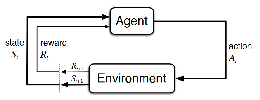
\includegraphics[width=3.5in]{agent_environment}
\caption{Agent-environment interaction \cite{sutton_barto_98}.}
\label{fig:agent_environment}
\end{figure}

Reinforcement learning (RL) problems consider an agent-environment interaction framework. Basics of reinforcement learning are mentioned in \cite{DBLP:journals/corr/MnihBMGLHSK16, DBLP:journals/corr/HasseltGS15, DRL:HumanLevelControl, DRL:Silver_2016, mnih-atari-2013}. As an in depth guide for reinforcement learning see \cite{sutton_barto_98}. The following part is about summarizing those background RL introductions. The agent (implementation of the learning algorithm) will interact with the environment (a Markov Decision Process). The interaction is continuous in time $t$, so the start state at time $t = 0$ is $s_0$ and a trajectory (decision sequence) looks like $(s_0, r_0) \rightarrow a_0 = (s_1, r_1) \rightarrow a_1 ... a_{t-1} = (s_t, r_t) \rightarrow a_t$. The agent environment interaction is graphically displayed in Fig. \ref{fig:agent_environment}. The agent will get a reward $R_t$ and a state $S_t$ from the environment and the environment will get an action $A_t$ from the agent. This action $A_t$ is a calculated decision based on the received reward $R_t$ and state $S_t$. After the environment received action $A_t$ it will return a state $S_{t+1}$ and a reward signal $R_{t+1}$. The agent tries to learn optimal behaviour through trial and error attempts. The agent wants to know which actions in which states get the most long-term reward and fit this knowledge into a policy representation. A few main problems of this RL framework are: 
\begin{itemize}
\item The agent only gets a numerical reward from the environment at the end of a decision-sequence. \\ $\sim$ \textit{Delayed Reward}
\item How should the reward be assigned to the different steps of a decision-sequence? \\ $\sim$ \textit{Credit Assignment Problem}
\item How to handle vast action- and state-spaces? \\ $\sim$ \textit{Generalization Problem}
\end{itemize}

This paper focuses heavily on the last mentioned problem. How to handle vast action- and state-spaces? In my bachelor thesis I also had the problem of high dimensional action- and state-spaces. I implemented a variant of table lookup Q-learning with a SQLite database for storing the agent experience. The agent should try to learn TicTacToe and Reversi (two board strategy games). Although the algorithm did OK for the TicTacToe (3x3 board) problem it completely failed for bigger game fields of TicTacToe or Reversi. The reason for failure was the exponential time increase proportional to the increasing dimensionality of action and state spaces. Q-functions cannot be represented in a table lookup, because the dimensions of most RL problems will lead to databases with more entries then particles in the universe (compare chess board positions and actions \cite{ertel_2009} S. 114 ff). One big and promising solution for this problem is function approximation in general and artificial neural networks in concrete.\\
 
A major goal of RL is to find a global optimal policy. A policy is a function which maps states to actions. This policy will additionally get a vector of parameters. The parameter-vector changes the policy output. This parametrisation of the policy function is called “function approximation” and Artificial Neural Networks are an approach for approximating a policy function. Combining ANN's with reinforcement learning algorithms have so far shown spectacular results e.g.: The Google DeepMind Team programmed an AI which plays Go (a very complex strategy board game) at human grandmaster level \cite{DRL:Silver_2016}. With this approximation the problem of vast action- and state-spaces can be solved. To optimise the parameter vector, methods  like Policy Gradient or Temporal Difference (e.g. Q-Learning) approaches are used. Applications like TD-Gammon by Gerald Tesauro proved that learning complex strategy games with Artificial Neural Networks is possible and promising.

\subsection{Q-learning}
Q-Learning (Watkins \cite{Watkins_1992}, 1989) is a reinforcement learning algorithm for agents to learn how to act optimally in controlled Markov decision processes. Watkins showed in his paper that Q-Learning converges to the optimum action-value with probability 1 so long as all actions are repeatedly sampled in all states and the action-value are represented discretely. We will describe the Q-Value update in detail now, because in a later chapter Q-Learning is a fundamental part of the implementation. The update rule of one-step Q-Learning is \cite{sutton_barto_98}:

\begin{equation} \label{equ:one step Q function}
\begin{split}
Q(S_t, A_t) \leftarrow & Q(S_t, A_t) + \alpha[R_{t+1} + \\
 & \gamma \max_a Q(S_{t+1},a) - Q(S_t, A_t)].
\end{split}
\end{equation}

This equation defines how to update a Q-value in one time step. Step size (or learning rate) $\alpha$ should be $0 \le \alpha < 1$ but often closer to $0$. This hyper parameter defines how much the agent can trust its experience. So if $\alpha$ is close to $0$ that means the agent should update its Q-values just a little bit in the direction of the temporal difference (TD), because the complete Q-Function is initialized randomly and the agent can't trust those values completely until a certain amount of updates is done. The temporal difference is the mathematical difference between two timely successive Q-Values: $\max_a Q(S_{t+1},a) - Q(S_t, A_t)$. TD represents the error between the two Q-Values, if TD is 0, then there is no difference between the states. Another hyper parameter is $\gamma$ which is a discounter. $\gamma$ defines how relevant future experience is for the agent. If $\gamma$ is close to 1 or is 1, then there is no discounting and every experience is equal important. If $\gamma$ is close to 0, then future experience gets more irrelevant proportional to the time distance. When $\gamma$ is 0, then no future experience is considered at all. $\max_a$ is a function which should return the highest Q-value for every possible action $a$ in state $S_{t+1}$ (also denoted as $S'$). 

\subsection{Loss Function}
A loss function $J(f)$ (or objective function) always defines how good or bad a function $f$ is. The result of a loss function is a scalar. Sometimes the loss function is also called a cost function, because if the resulting scalar is a high value, then its like the cost of function $f$ is high. There are several different loss functions for different tasks. In supervised learning tasks for example linear regression a mean squared error (MSE) loss is used. Mathematically MSE loss looks like this: 

\begin{equation*}
J_D(\Theta) = \frac{1}{2m} \sum^m_{i=1}(h_\Theta(x^{(i)}) - y^{(i)})^2).
\end{equation*}

\begin{figure}[!t]
\centering
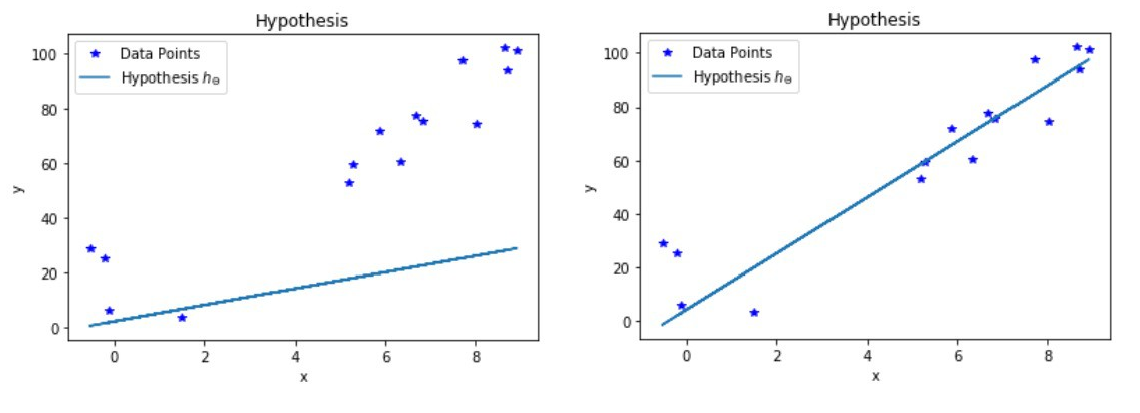
\includegraphics[width=3.5in]{linear_regression_model_fit}
\caption{Fitting a linear hypothesis with linear regression.}
\label{fig:linear_regression_model_fit}
\end{figure}

$D$ is the data or the training set which includes all training values $x$ and all target values $y$ (labels). $m$ is the amount of training examples inside $D$. $\Theta$ is a parameter vector containing several different Parameters $(\theta_0, \theta_1, ..., \theta_n)$. Parameter vector $\Theta$ affects the output of the linear hypotheses $h_\Theta$. Using the MSE loss function $J_D(\Theta)$ and a gradient descent method it is possible to fit the linear hypothesis to the given data. Fig. \ref{fig:linear_regression_model_fit}. displays the start point and the result of a linear regression as described above. The blue data points are not measured data, these points are calculated with a Gaussian normal distribution. So to all $y$ values a Gaussian noise is added. The left graph is the not fitted random initialized hypothesis $h_\Theta$ and the right graph is the fitted hypothesis after 400 iterations using MSE loss and gradient descent. For completeness the parameter vector $\Theta$ is optimized and so the hypothesis  will fit the data, because the hypothesis $h_\Theta$ is dependent on $\Theta$. \\

In reinforcement learning tasks loss functions look and behave similar as in supervised learning. Later we will examine a successful Q-Learning implementation with a neural network as function approximation using a loss function $L_i(\theta_i)$ and to understand this loss function it is helpful to understand the example loss function given above.

\subsection{Batch vs. Stochastic Gradient Decent}
In the privious chapter we already talked about gradient descent metodes, but we did not defined how gradient descent works. Now we will explain two different gradient descent methodes in detail. The following differentiation of batch and stochastic gradient descent is based on \cite{bottou-bousquet-2008} and \cite{bottou-2010}: In general gradient methods are used to optimize a function respective to its partial derivatives. A parameter update with batch gradient descent will consider the whole training set for its calculation. So in large scale machine learning problems there are training sets with several millions or billions of examples. For every update step the batch gradient descent calculates the sum of the partial derivatives in respective to all examples. To find the minimum of a function multiple update steps are needed. Batch gradient descent will have an exponential computational cost for larger machine learning problems. \\

A Solution for this problem is the stochastic gradient descent. Instead of computing the gradient of the function exactly, each iteration (update step) estimates the gradient on the basis of a single randomly picked example. The trade-off between batch and stochastic gradient descent is that batch gradient descent achieves linear convergence, when the initial estimate is close enough to the optimum and when the gain of the discounting factor is sufficiently small. The stochastic gradient descent will not converge to a minimum like batch gradient descent does, rather the parameters which are updated will oscillate around the minimum but will may never converge to the minimum. But often the stochastic gradient descent gets the parameters close to the minimum much faster than batch gradient descent. \\

\begin{figure}[!t]
\centering
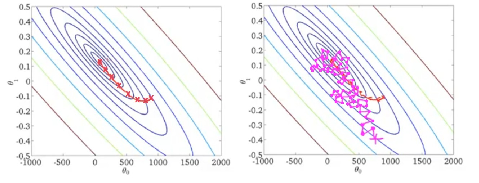
\includegraphics[width=3.5in]{gradient_plots}
\caption{Contour plots of cost function $J(\theta)$ with marked batch (left) and stochastic gradient descent (right) \cite{ng_2017}.}
\label{fig:gradient_plots}
\end{figure}

\begin{algorithm}
\caption{Stochastic gradient descent \cite{ng_2017}} \label{alg:stochastic gradient descent}
\begin{algorithmic}
\STATE Randomly shuffle (reorder) training examples
\REPEAT
\FOR{ $i := 1, ... ,m$}
	\FOR{$j := 0, ... , n$}
	\STATE $\theta_j := \theta_j - \alpha (h_\theta(x^{(i)}) - y^{(i)}) x^{(i)}_j$
	\ENDFOR
\ENDFOR
\UNTIL{1-10 times}


\end{algorithmic}
\end{algorithm}

Figure \ref{fig:gradient_plots} illustrates how batch and stochastic gradient descent converge to a minimum. The coloured ovals define the contour of a cost function $J(\theta)$. The cost function is minimal in the middle of the smallest oval and gets higher in the outer ovals. The parameters $\theta_0$ and $\theta_1$ are two parameters of a parameter vector $\theta$. Those parameter values will change the cost of function $J(\theta)$. In the left part of figure \ref{fig:gradient_plots} parameters $\theta$ updated by batch gradient descent converges "relatively straight" to a minimum after several iterations. Whereas in the right part of figure \ref{fig:gradient_plots} parameters $\theta$ updated by stochastic gradient descent are in general moved in the direction of the minimum but not always and in the end the parameters are wondering around close to the minimum.

Algorithm \ref{alg:stochastic gradient descent} is a pseudocode example of stochastic gradient descent from Andrew Ng \cite{ng_2017}. The term $m$ denotes the amount of training examples, $n$ is the amount of parameters $\theta$, hyper parameter $\alpha$ is the step size or learning rate which we already mentioned in chapter Q-learning and $h_\theta(x^{(i)}) - y^{(i)}$ is a part of the error term mentioned in chapter loss function. For a concrete example with $m = 300.000.000,00$ training examples the algorithm \ref{alg:stochastic gradient descent} will update all parameters $\theta_n$ for every training example. So in one single stochastic gradient descent step the parameter vector $\Theta = \theta_0, ..., \theta_n$ is updated $m$ times. Batch gradient descent will in contrast calculate an update of all parameters $\theta_n$ considering all training examples at once and then just performing one single batch gradient descent update of the parameter vector $\Theta$.

\section{Artificial Neural Networks (ANN's)}
In neural networks in general between the output and the input layers are hidden layers. If there is more then one hidden layer between input and output layer, then the neural network is called a deep neural network.

\subsection{Convolutional Neural Network (CNN/ConvNet)}

\begin{figure}[!t]
\centering
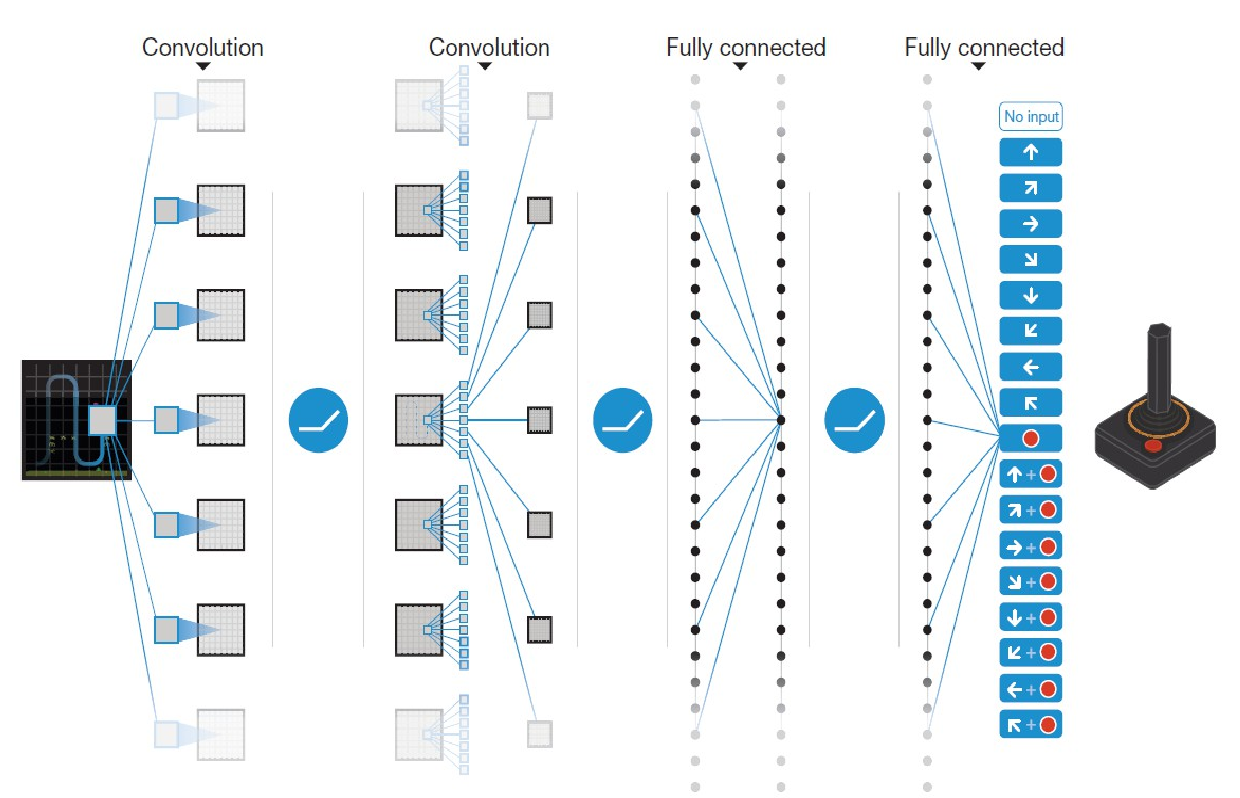
\includegraphics[width=3.5in]{conv_net}
\caption{Schematic illustration of the convolutional neural network \cite{DRL:HumanLevelControl}.}
\label{fig:conv_net}
\end{figure}

To better understand the later experiment \cite{mnih-atari-2013} (Deep Q-network) it is helpful to get into CNN's first. Knowledge base of this chapter is a Stanford class CS231n about "Convolutional Neural Networks for Visual Recognition" \cite{KarpathyCNN}. A convolutional neural network is a specific ANN which assumes that every input is an image. This assumption allows to reduce the amount of parameters and so improve the performance for image processing with CNN's in contrast to more general ANN's. More general because ANN's don't assume a specific input. A CNN consists of layers. There are different kinds of layers: input layer (INPUT), convolutional layer (CONV), rectified linear unit layer (RELU), pooling layer (POOL), fully connected layer (FC) and an output layer. Some of these layers can appear multiple times. A simple ConvNet architecture for classification could be INPUT $\rightarrow$ CONV $\rightarrow$ RELU $\rightarrow$ POOL $\rightarrow$ FC. In the following every different layer will be explained in detail.

\paragraph{The Input layer} can be high dimensional sensory data. Considering the Atari 2600 arcade gaming environment \cite{DBLP:journals/corr/MnihBMGLHSK16, DBLP:journals/corr/HasseltGS15, DRL:HumanLevelControl} the input is a video stream of pixels at different time steps. At time step $t$ a video signal reduces to just an image of pixels and the complete sequence of images at all time steps equals the video signal. There is still more then the raw pixels from the video stream like the score value at each time step \cite{DRL:HumanLevelControl}. In terms of reinforcement learning the score signal is a reward signal and the video stream at each time step describes the state in which the agent is in. Another example is the CIFAR-10 dataset which contains images of shape 32x32x3 (32 wide, 32 high, 3 color channels).

\begin{figure}[!t]
\centering
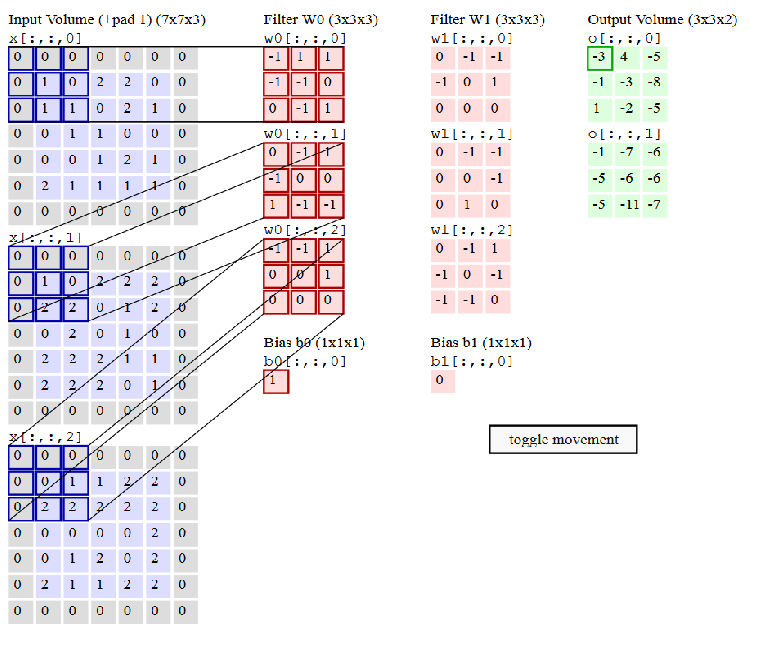
\includegraphics[width=3.5in]{convolutional_layer}
\caption{Computation inside a convolution layer \cite{KarpathyCNN}.}
\label{fig:convolutional_layer}
\end{figure}

\paragraph{The convolution layer} is the most computationally expensive layer, because much matrix multiplications are performed on raw data (not reduced data expect preprocessing). In general this layer applies filters on input images. A filter is a window with fixed size for the CIFAR-10 example the filters could have a size of 5x5x3. These filters are shifted around the width and height of the input images and for every position a matrix multiplication between the input image and the filter is performed. The matrix multiplication results in scalar values stored in a result matrix (feature map). Every filter produces an own feature map. Filters represent the weights of CNN's. For every filter there is an additional bias weight which need to be considered inside the computation. The output of this layer is controlled by three hyperparameters: depth, stride and zero-padding.

\begin{itemize}
\item Depth
\item Stride
\item Zero-padding
\end{itemize}    

A filter can be a representation for edges, lines or other shapes. A combination of those low level filters results in more complex filters like an eye or an ear. Those low and high level filters are like extracted features from the CNN. The computation inside a convolution layer is represented in Fig. \ref{fig:convolutional_layer}. Three input matrices of shape 7x7 are independently drawn, because each matrix represents the red, green or blue color channel so the input layer has a shape of 7x7x3 (7 wide, 7 high, 3 color channels). The outer lines (matrix borders) are all zero 

\paragraph{The rectified linear unit layer} will apply an elementwise activation function, such as the $max(0,x)$ thresholding at zero. If $max(0,x)$ gets values below zero then it will return just zero and if the values are greater then zero $max$ will return the value itself. The blue circles in Fig. \ref{fig:conv_net} with a white line after CONV and FC layers represent the RELU activation function. The $max(0,x)$ rectifier is used for deep learning rather then e.g. the logistic sigmoid, because of better practical efficiency.

\paragraph{The pooling layer} 

\paragraph{The output layer} Aim of the CNN is to predict which of 10 different CIFAR classes an image belongs to.

\section{Playing Atari with Deep Reinforcement Learning}
The paper from DeepMind Technologies is about a deep learning model to successfully learn control policies directly from high-dimensional sensory input using reinforcement learning \cite{mnih-atari-2013}. They defined the model as a convolutional neural network (CNN). This CNN is trained with a variant of Q-learning. Input of the CNN is row pixels and output is a value function estimating future rewards. They apply this deep learning model to seven Atari 2600 games from the Arcade Learning Environment, with no adjustment of the architecture or learning algorithm. Result of this experiment is that it outperforms all previous approaches on six of the games and surpasses a human expert on three of them. 

\subsection{Deep Reinforcement Learning}
The following subsection is an in depth explanation of the experiment done in paper "Playing Atari with Deep Reinforcement Learning" \cite{mnih-atari-2013}. Inside the deep Q-learning algorithm (see Algorithm \ref{alg:deep q learning}) every concept explained in previous chapters are involved. This algorithm describes a deep Q network (DQN). A deep Q network is a combination of a convolutional neural networks and the reinforcement learning algorithm Q-learning. The problem setting is a Markov Decision Process defined by the Atari 2600 games emulator. The algorithm aims to learn an optimal policy like reinforcement learning agents always try to in an MDP environment.

\begin{equation} \label{equ:loss functions}
L_i(\theta_i) = \mathbb{E}_{s,a \sim \rho(\cdot)} [(y_i - Q(s,a;Q_i))^2]
\end{equation}

Furthermore a sequence of loss functions displayed in equation \ref{equ:loss functions} is used by Mnih et al. 2013 \cite{mnih-atari-2013}. The core of the loss function equation \ref{equ:loss functions} is pretty similar to the Q-function of Sutton and Barto \cite{sutton_barto_98} equation \ref{equ:one step Q function} or the original from Watkins \cite{Watkins_1992}. The similarity appears because of the objective definition in Reinforcement Learning problems. RL objective is to maximize the accumulated rewards over time. This RL objective is mathematically formalized either in Sutton and Bartos one step Q-update rule (equation \ref{equ:one step Q function}) and in Mnih et al. equation of loss functions (equation \ref{equ:loss functions}).

\begin{equation} \label{equ:gradient loss}
\begin{split}
\nabla_{\theta_i} L_i (\theta_i) = & \mathbb{E}_{s,a \sim \rho(\cdot);s'\sim \mathcal{E}} [(r + \gamma \max_{a'} Q(s',a';\theta_{i-1}) \\
 & - Q(s,a;\theta_i)) \nabla_{\theta_i} Q(s,a;\theta_i)]
\end{split}
\end{equation}

These loss functions are optimized by a stochastic gradient descent update referenced in equation \ref{equ:gradient loss}. 

\begin{equation} \label{equ:true Q-value-function}
Q^*(s,a) = \mathbb{E}_{s' \sim \mathcal{E}} [r + \gamma \max_{a'} Q^* (s',a') |s,a]
\end{equation}

Mnih et al. used a convolutional neural network as function approximation to estimate the true Q-value-function $Q^*(s,a)$ defined in equation \ref{equ:true Q-value-function}. So the approximation is a Q-function $Q(s,a;\theta)$ with an additional parameter vector of weights $\theta$. The deep Q-learning algorithm optimizes the weights of the convolutional neural network function approximation for an nearly optimal approximation of $Q(s,a;\theta) \approx Q^*(s,a)$. Initially the weights of the CNN are randomly initialized, so the entries (neurons) will not behave exactly homogeneous.

\begin{algorithm}
\caption{Deep Q-learning with Experience Replay \cite{mnih-atari-2013}} \label{alg:deep q learning}
\begin{algorithmic}
\STATE Initialize replay memory $\mathcal{D}$ to capacity $N$
\STATE Initialize action-value function $Q$ with random weights
\FOR{ episode $= 1, M$}
	\STATE Initialise sequence $s_1 = \{x_1\}$ and preprocessed \\
	\qquad sequenced $\phi_1 = \phi(s_1)$
	\FOR{$t = 1,T$}
		\STATE With probability $\epsilon$ select a random action $a_t$
		\STATE otherwise select $a_t = \max_a Q^* (\phi(s_t),a;\theta)$
		\STATE Execute action $a_t$ in emulator and observe reward $r_t$ \\
		\qquad and image $x_{t+1}$
		\STATE Set $s_{t+1} = s_t, a_t, x_{t+1}$ and preprocess $\phi_{t+1} =
		\phi(s_{t+1})$
		\STATE Store transition $(\phi_t,a_t,r_t,\phi_{t+1})$ in $\mathcal{D}$
		\STATE Sample random minibatch of transitions \\
		\qquad $(\phi_j,a_j,r_j,\phi_{j+1})$ from $\mathcal{D}$
		\STATE \medskip Set $y_j = \begin{cases} 
			r_j \qquad \qquad \quad \text{for terminal } \phi_{j+1} \\
			r_j + \gamma \max_{a'} Q(\phi_{j+1},a';\theta) \\
			\qquad \qquad \qquad \text{for non-terminal} \phi_{j+1}		
		\end{cases}$
		\STATE Perform a gradient descent step on $(y_j - 
		Q(\phi_i,a_j;\theta))^2$ \\ \qquad according to equation
		\ref{equ:gradient loss}
	\ENDFOR
\ENDFOR
\end{algorithmic}
\end{algorithm} 

\subsection{Experiment results}

The deep Q-learning algorithm from the previous subsection achieved better performance than an expert human player on the Atari games Breakout, Enduro and Pong and achieves close to human performance on Beam Rider. The human expert outperformed the DQN in games like Q*bert, Seaquest and Space Invaders, because the games are more challenging in terms of the DQN needs to find a strategy that extents over long time scales. Nevertheless the DQN outperforms other RL algorithms like Sarsa and Contingency. These results are summarized in table \ref{fig:result_table_dqn}. The first row of the table is a random agent which acts randomly without any RL algorithm. The next 4 rows are already described previously. The last 3 rows compare the best DQN results with a evolutionary policy search approach. 

\begin{figure}[!t]
\centering
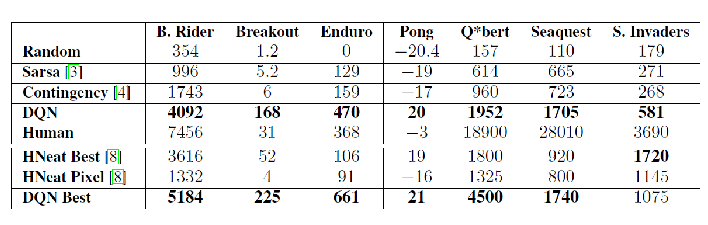
\includegraphics[width=3.5in]{result_table_dqn}
\caption{DQN results in Atari 2600 emulator \cite{mnih-atari-2013}.}
\label{fig:result_table_dqn}
\end{figure}

\section{Discussion \& Conclusion}
Even if the DQN from Mnih et al. 2013 outperforms a human in several Atari 2600 games, there are still games where the human is unbeatable. The paper "Deep Reinforcement Learning with Double Q-Learning" aims to determine if the recent DQN (Deep Q Network) algorithm, which combines Q-learning with a deep neural network, suffers from substantial overestimations in some games in the Atari 2600 domain \cite{DBLP:journals/corr/HasseltGS15}. Furthermore the Google DeepMind contributors point out how the Double Q-learning algorithm can be generalized to work with large-scale function approximation to successfully reduce the DQN overoptimism, resulting in more stable and reliable learning. Finally they propose a specific adaptation to the DQN algorithm and show that the resulting algorithm (Double DQN) not only reduces the observed overestimation, as they hypothesized, but that this also leads to much better performance on several Atari 2600 games. \\

The main paper of Mnih et al. 2013 \cite{mnih-atari-2013} is the foundation for another very similar paper "Human-level controll through deep reinforcement learning" \cite{DRL:HumanLevelControl}. The paper is about how to reach human-level control through a deep Q-network, that can learn successful policies directly from high-dimensional sensory inputs using end-to-end reinforcement learning. The deep Q-network agent is tested on the challenging classic Atari 2600 game environment. The result of this test demonstrated that the deep Q-network agent, receiving only the pixels and the game score as inputs, was able to surpass the performance of all previous algorithms and achieve a level comparable to that of a professional human games tester across a set of 49 games, using the same algorithm, network architecture and hyperparameters. \\

Another promissing approach using artificial neural networks as function approximation is created by scientists from Google DeepMind and Montreal Institute for Learning Algorithms, they introduced asynchronous deep learning algorithms \cite{DBLP:journals/corr/MnihBMGLHSK16}. These asynchronous algorithms are based on four standard reinforcement learning algorithms: One-step Q-learning, one-step Sarsa, n-step Q-learning and advantage actor-critic. We already mentioned one-step Q-learning in a previous section. The paper explains the background of reinforcement learning and how the asynchronous reinforcement learning methods works. The study was approved by an experiment in an Atari 2600 evaluation environment. All four asynchronous algorithms where tested within the test environment. The Atari 2600 environment tests where used to compare the performance of the four algorithms. The main finding of this study is that all four asynchronous deep reinforcement learning algorithms are able to train neural network controllers on a variety of domains in a stable manner. In addition their results show that stable training of neural networks through reinforcement learning is possible with both value-based and policy-based methods, off-policy as well as on-policy methods, and in discrete as well as continuous domains. \\

So far we only mentioned RL environments given by the Atari 2600 emulator, but what if we would define an extremely high dimensional board game like GO as an RL environment? The paper from D. Silver et al. 2016 concerns two different algorithm approaches for deep reinforcement learning \cite{DRL:Silver_2016} of the board game GO. The first approach uses 'value networks' to evaluate board positions and 'policy networks' to select moves. These deep neural networks are trained by a novel combination of supervised learning from human expert games and reinforcement learning from games of self-play. They proof through experiments that this deep RL algorithm approach is capable of playing Go at the level of state-of-the-art Monte Carlo tree search. The second deep RL approach is a new seach algorithm that combines Monte Carlo simulation with value and policy networks. They used this search algorithm inside the application AlphaGo and the application achieved a 99.8\% winning rate against other Go programs and it defeated the human European Go champion by 5 games to 0. \\

To close out the paper and give a final statement we will summarize this paper in short. We explained what reinforcement learning in general is, what the problems of reinforcement learning are, how to solve the problem of high dimensionality with function approximation using convolutional neural networks as function approximation, what convolutional neural networks are, how loss functions look and how they define the agent objective, what the difference between the optimization methods batch gradient decent and stochastic gradient descent are and we explained how all these concepts are used by Mnih et al. 2013 \cite{mnih-atari-2013} to create a deep RL algorithm which outperforms human level gameplay in several Atari 2600 games. Convolutional neural networks which are more specialized artificial neural networks combined with RL methods produce powerful approaches to learn human level or above human level strategies in most of Atari 2600 like games or GO without changing hyperparameters or network architecture mostly. In several years the deep RL algorithms may beat humans in every Atari 2600 game. 

% use section* for acknowledgment
% \section*{Acknowledgment}


%The authors would like to thank...





% trigger a \newpage just before the given reference
% number - used to balance the columns on the last page
% adjust value as needed - may need to be readjusted if
% the document is modified later
%\IEEEtriggeratref{8}
% The "triggered" command can be changed if desired:
%\IEEEtriggercmd{\enlargethispage{-5in}}

% references section

% can use a bibliography generated by BibTeX as a .bbl file
% BibTeX documentation can be easily obtained at:
% http://mirror.ctan.org/biblio/bibtex/contrib/doc/
% The IEEEtran BibTeX style support page is at:
% http://www.michaelshell.org/tex/ieeetran/bibtex/
\bibliographystyle{IEEEtran}
% argument is your BibTeX string definitions and bibliography database(s)
\bibliography{paper}
%
% <OR> manually copy in the resultant .bbl file
% set second argument of \begin to the number of references
% (used to reserve space for the reference number labels box)

% that's all folks
\end{document}


